\section{中性子検出器}
実験では中性子を検出する必要があるが、中性子は電荷をもたないためそれを直接検出することは困難である。そこで、強い相互作用による反応で生じた荷電粒子を検出することで、間接的に中性子を検出する方法をとる。この節では実験で用いた中性子検出器の原理と仕組みを説明する。

検出に利用する反応は検出する中性子のエネルギーによって様々であるが、今回の実験で用いた熱中性子($\sim$ 25 meV)の場合、次のような中性子捕獲反応が主に利用される:
\begin{align}
&\ce{^3He} + \ce{n} \to \ce{^3H}+\ce{p} + 0.705 \, \mathrm{MeV} \label{Kasuya_3He} \\
&\ce{^6Li} + \ce{n} \to \ce{^3H}+\ce{^4He}+4.78 \, \mathrm{MeV} \label{Kasuya_6Li}
\end{align}

\subsection{$\ce{^3He}$ガスを充填した比例計数管}
今回の実験では入射する中性子の時間情報と個数を知る必要がある。そこで入射粒子の数を1つずつ数える微分型の検出器として、$\ce{^3He}$ガスを充填した比例計数管を用いた。

\paragraph{検出原理}
検出には(\ref{Kasuya_3He})の反応が利用される。反応で生じた荷電粒子が気体中を進むと、軌道上の気体分子が電離してイオン・電子対が生じる。電場をかけてそれらを集めることで、信号として読み取ることができる。エネルギー25 meVの中性子に対する$\ce{^3He}$原子核の断面積は5333 barnである~\cite{JENDL}。
%低エネルギーでこの断面積は中性子の速度に反比例することが知られている[]ため、エネルギー$E$(meV)の中性子に対する$\ce{^3He}$原子核の断面積は$\sigma(E)=5333\sqrt{25/E}$(barn)となる。
これは気体の中では非常に大きく、効率よく中性子の数を数えることができる。

\paragraph{検出の仕組み}
円筒形の容器の中に$\ce{^3He}$ガスが封入されており、高電圧がかけられた中心のワイヤと接地された容器の内壁がそれぞれ陽極と陰極として機能する。$\ce{^3He}$ガスは(\ref{Kasuya_3He})の反応によって荷電粒子を発生させる中性子有感物質であると共に、この荷電粒子によって電離して信号を増幅させる被電離気体の役割を果たす。

\begin{figure}[h]
\begin{minipage}{0.45\hsize}
\begin{center}
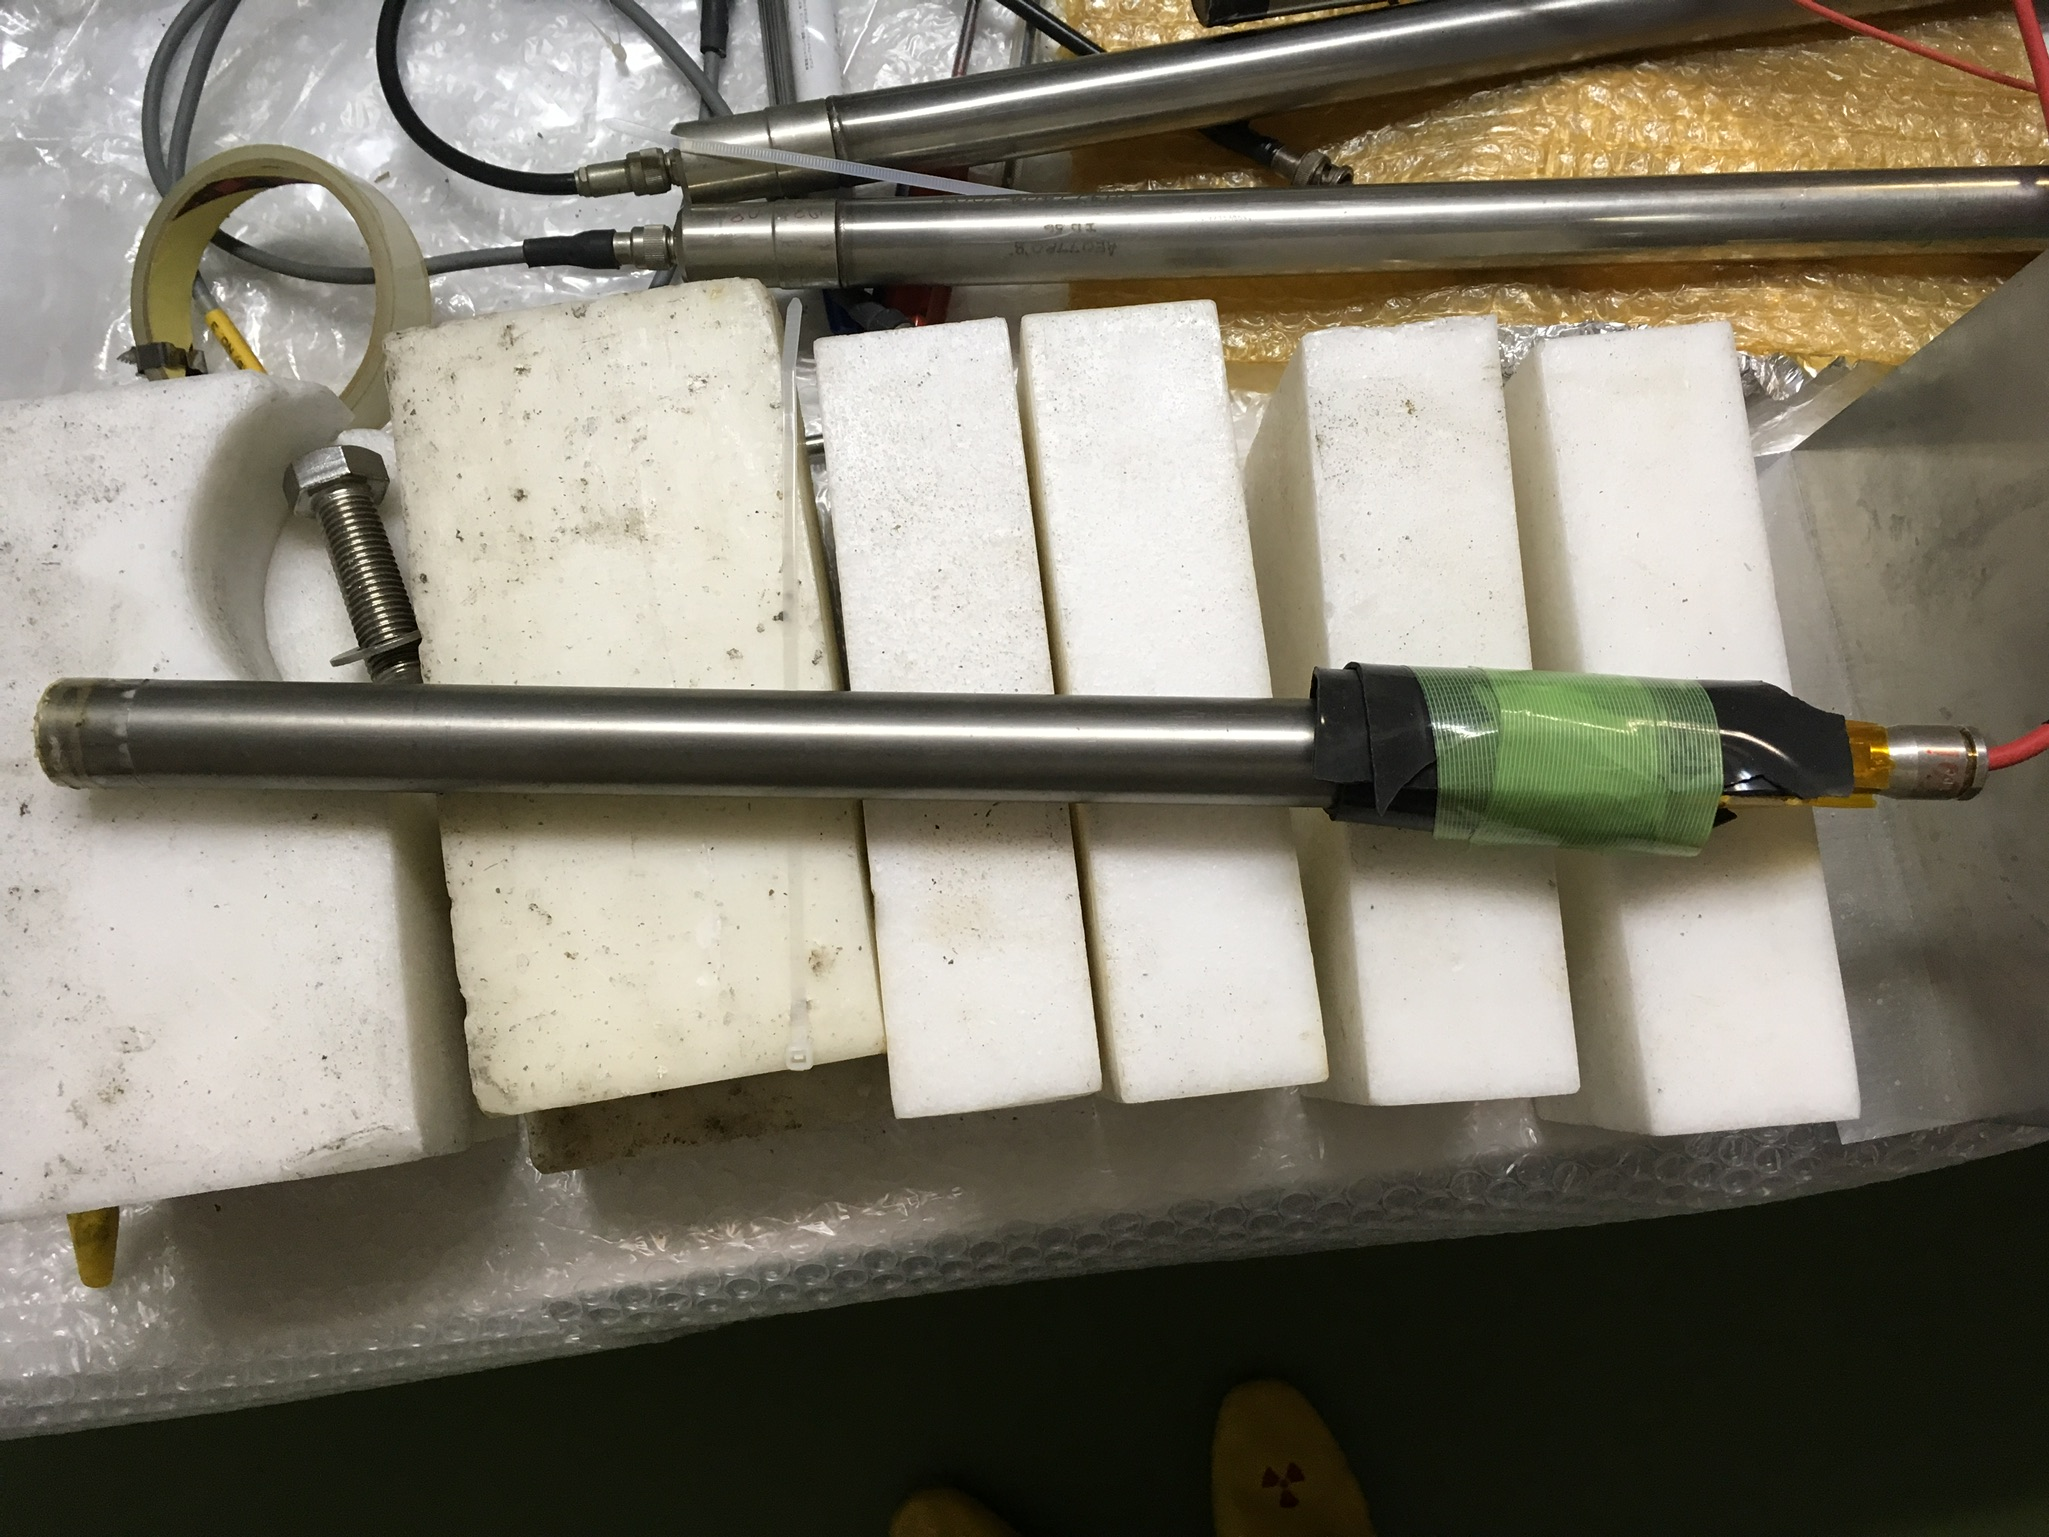
\includegraphics[height=4.5cm]{detector/detector_photo1.jpg}
\subcaption{写真}
\end{center}
\end{minipage}
\begin{minipage}{0.55\hsize}
\begin{center}
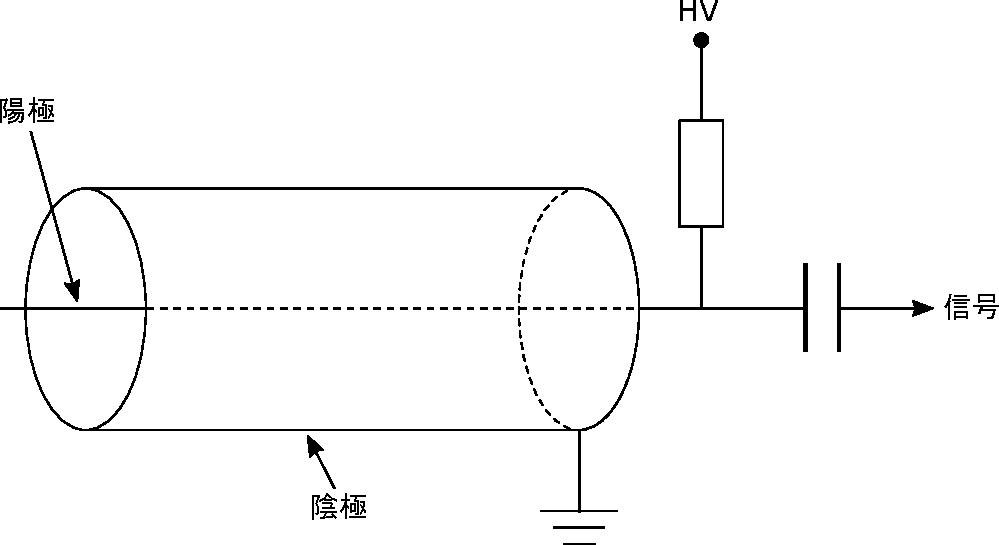
\includegraphics[height=4.5cm]{detector/detector_fig1.pdf}
\subcaption{模式図}
\end{center}
\end{minipage}
\caption{比例計数管}
\end{figure}

\subsection{RPMT検出器}
予備実験では入射する中性子の2次元的な位置情報を知る必要がある。そこで2次元位置感度型検出器として、RPMT検出器を用いた。

\paragraph{検出原理}
検出には(\ref{Kasuya_6Li})の反応が利用される。反応で生じた荷電粒子によってシンチレータ中の原子や分子が励起され、下の準位に戻る際に光が放出される(シンチレーション光)。生じた光は光電子増倍管で増幅され信号として取り出される。使用するRPMTではシンチレータに$\ce{^6LiF}/\ce{ZnS}$を用いる。$\ce{^6LiF}/\ce{ZnS}$は発光量が大きくガンマ線感度が低いことから、中性子の検出に適している。

\paragraph{検出の仕組み}
RPMTは$\ce{^6LiF}/\ce{ZnS}$シンチレータにPSPMT(Position Sensitive PMT,位置分解能をもつ光電子増倍管)を取り付けた構造をしている。PSPMTは内部にX軸Y軸のメッシュ状の読み取り用電極をもち、電荷分割法により中性子の検出位置を$x/L=Q_2/(Q_1+Q_2)$で求めることができる。ここで$L$は電極の全長、$x$は検出位置、$Q_1,Q_2$は2本のケーブルからの出力電荷である。検出位置はX軸Y軸について1024 ch$\times$1024 chの分解能で計測され、チャンネル幅は$1 \, \mathrm{ch}$あたり$0.119\pm0.002 \, \mathrm{mm}$と報告されている~\cite{KUANS_yamashita}。

\begin{figure}[h]
\begin{minipage}{0.5\hsize}
\begin{center}
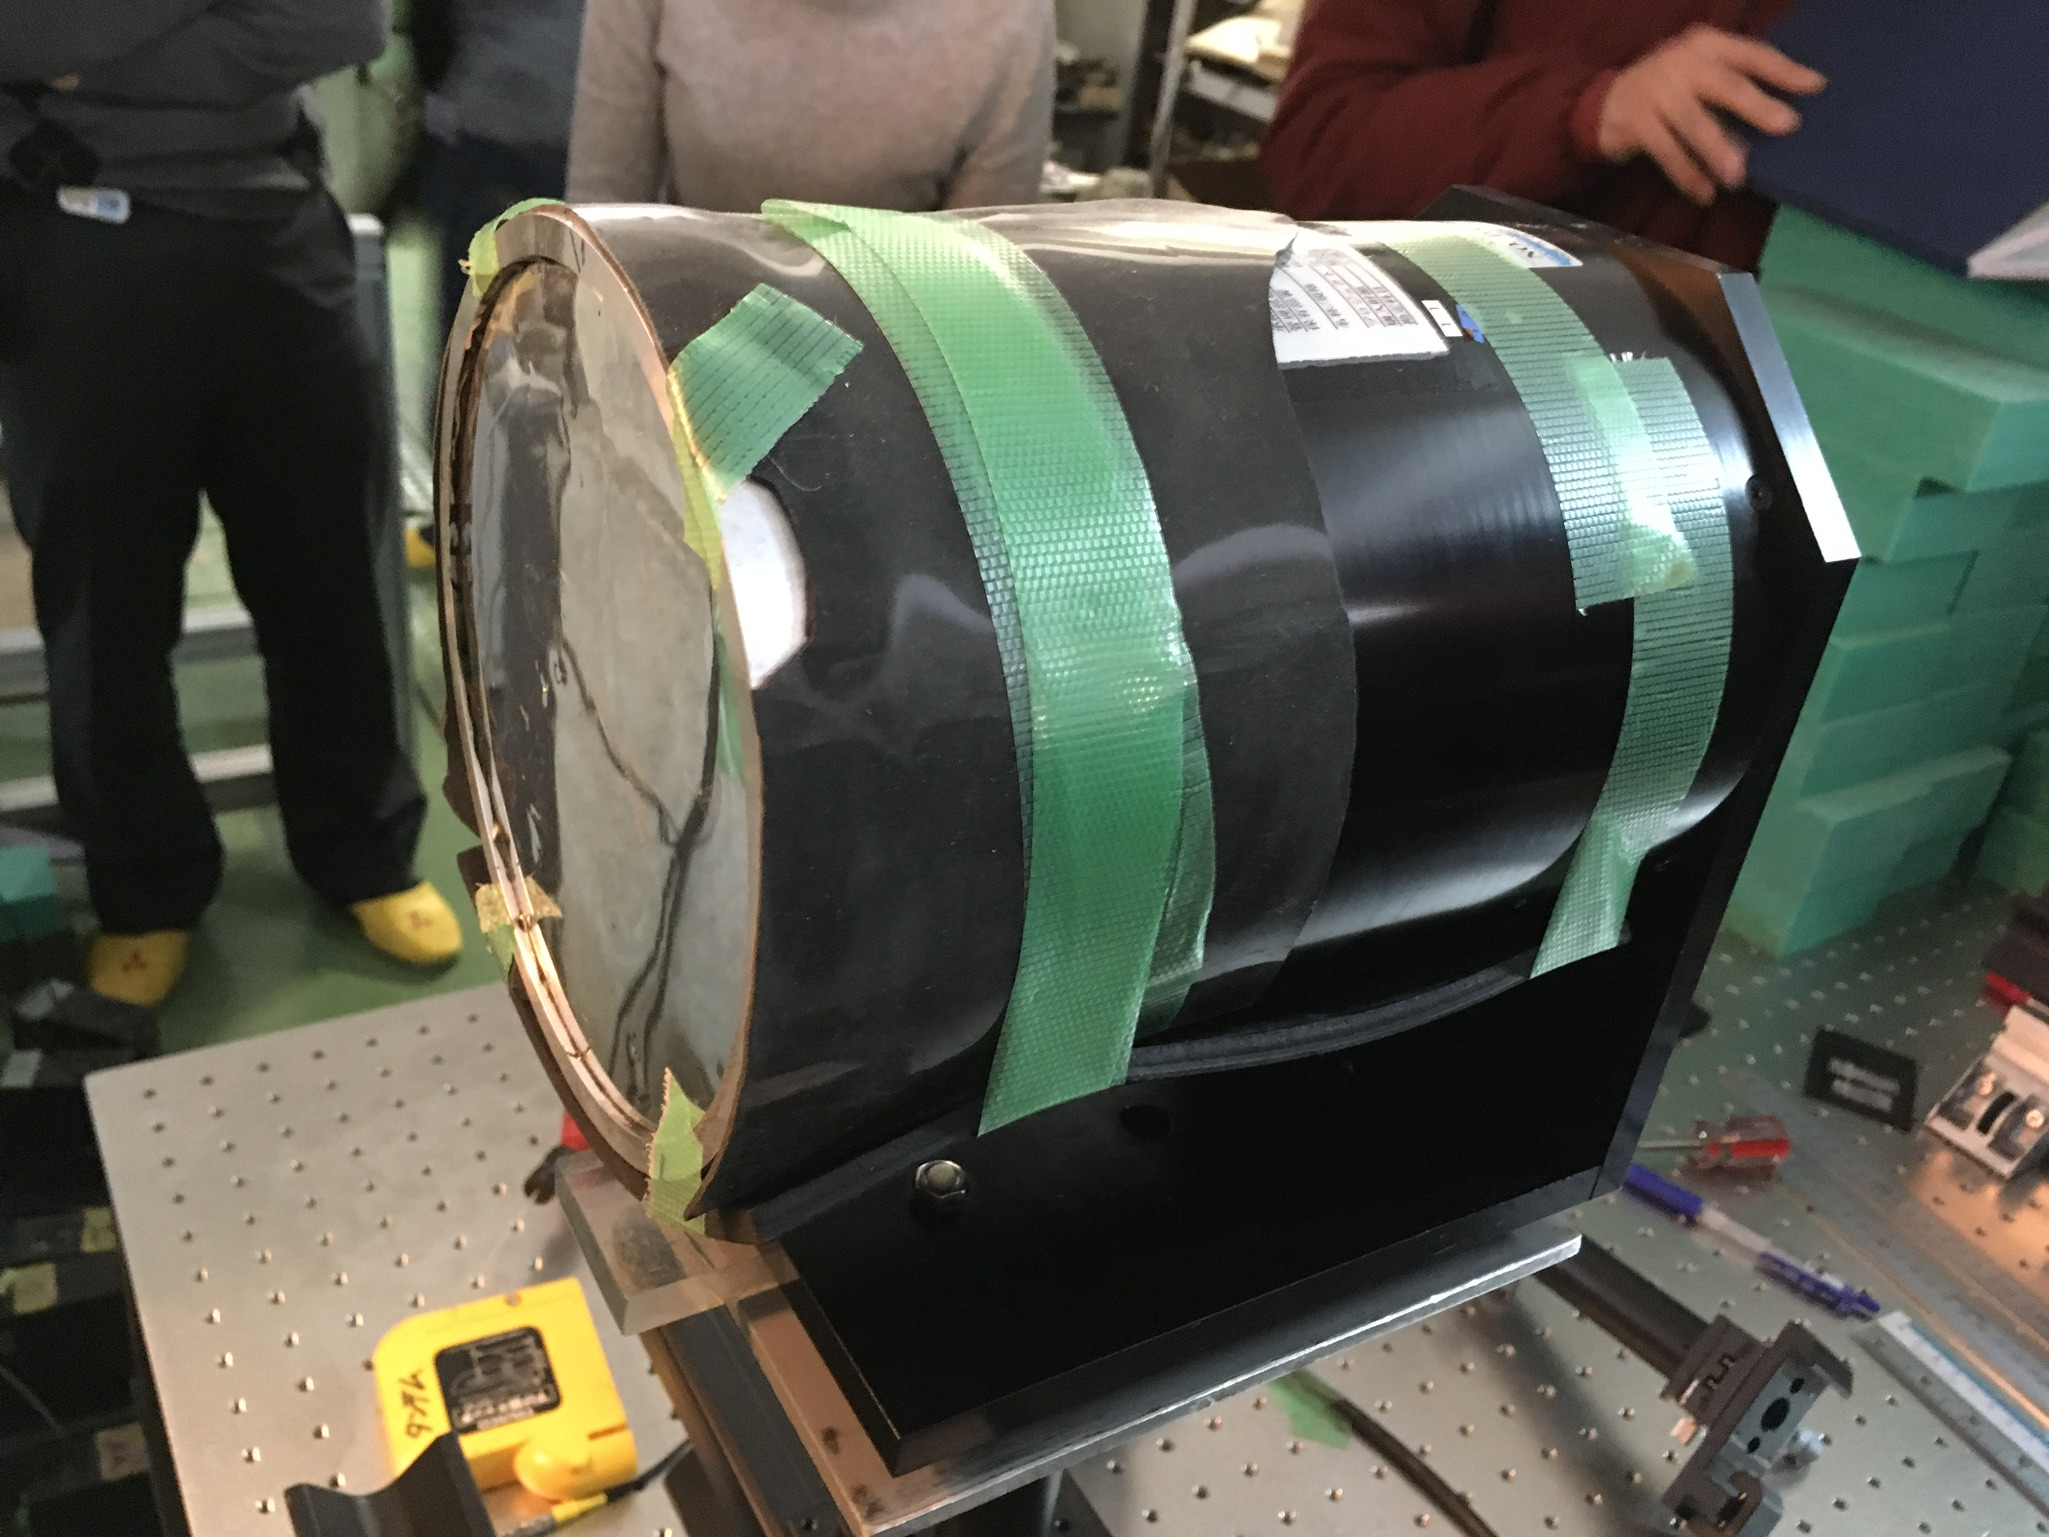
\includegraphics[height=4.5cm]{detector/detector_photo2.jpg}
\subcaption{写真}
\end{center}
\end{minipage}
\begin{minipage}{0.5\hsize}
\begin{center}
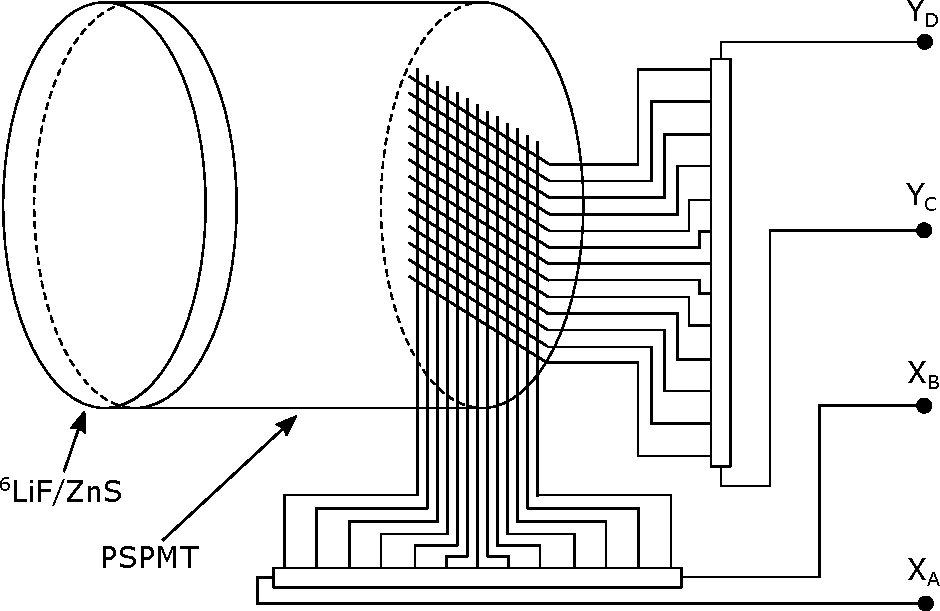
\includegraphics[height=4.5cm]{detector/detector_fig2.pdf}
\subcaption{模式図}
\end{center}
\end{minipage}
\caption{RPMT検出器}
\end{figure}
\begin{figure}[h]
\begin{minipage}{0.5\hsize}
\begin{center}
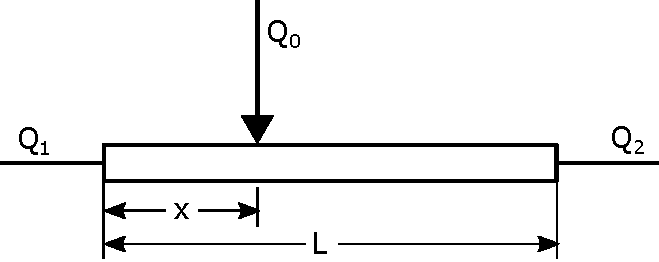
\includegraphics[width=6.5cm]{detector/detector_fig3.pdf}
\caption{電荷分割法}
\end{center}
\end{minipage}
\end{figure}





